\chapter{Arquitectura de la solución}\label{arquitectura}

Luego de analizar las necesidades del proyecto y el estado actual de la industria frente al desafío, el siguiente paso es establecer una arquitectura base con la cual definir las partes más relevantes del sistema. En la figura \ref{arqui} se pueden apreciar las 3 secciones relevantes y detalladas en las siguientes secciones.

\begin{figure}[H]
	\centering
	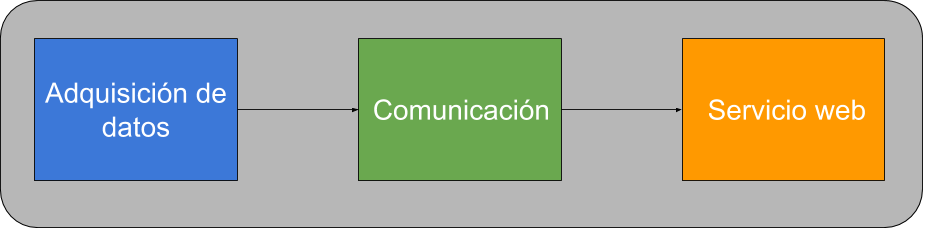
\includegraphics[scale=0.43]{figuras/arquitectura/arqui.png}
	\caption{Arquitectura referente}
	\label{arqui}
\end{figure}

\newpage
\section{Adquisición de datos}
Una primera necesidad del proyecto es la obtención y procesamiento de los datos, en una primera instancia se omitirá la definición del almacenamiento, permitiendo enfocar los esfuerzos en la selección de sensores, su interconexión y la plataforma que sustente su funcionamiento. Algunos de los requisitos en este apartado son:

\begin{enumerate}
	\item \textbf{Variedad:}
	Considerando la gama de enfermedades que se podrían cubrir, es importante contemplar una plataforma que permita trabajar con gran cantidad sensores.
	\item \textbf{Comodidad:}
	A raíz de que este apartado es el único que tendrá contacto con el paciente es importante pensar en el confort ofrecido, descartando opciones que afecten este apartado, como placas demasiado grandes o pesadas.
	\item \textbf{Flexibilidad:}
	Al estar en un proceso iterativo en búsqueda de opciones, un factor a considerar es la flexibilidad que nos puedan ofrecer las distintas opciones, permitiéndonos realizar cambios importantes sin afectar en gran medida las decisiones ya tomadas.
\end{enumerate}

\newpage
\section{Comunicación}
En el apartado 

\newpage
\section{Servicio web}

